\documentclass[tikz,border=8pt]{standalone}
\usepackage{amsmath}
\usetikzlibrary{arrows.meta,calc,patterns,decorations.pathreplacing}
\definecolor{ink}{HTML}{17324D}
\definecolor{blue}{HTML}{1877B8}
\definecolor{orange}{HTML}{D97706}
\definecolor{green}{HTML}{16856B}
\definecolor{red}{HTML}{C24156}
\begin{document}
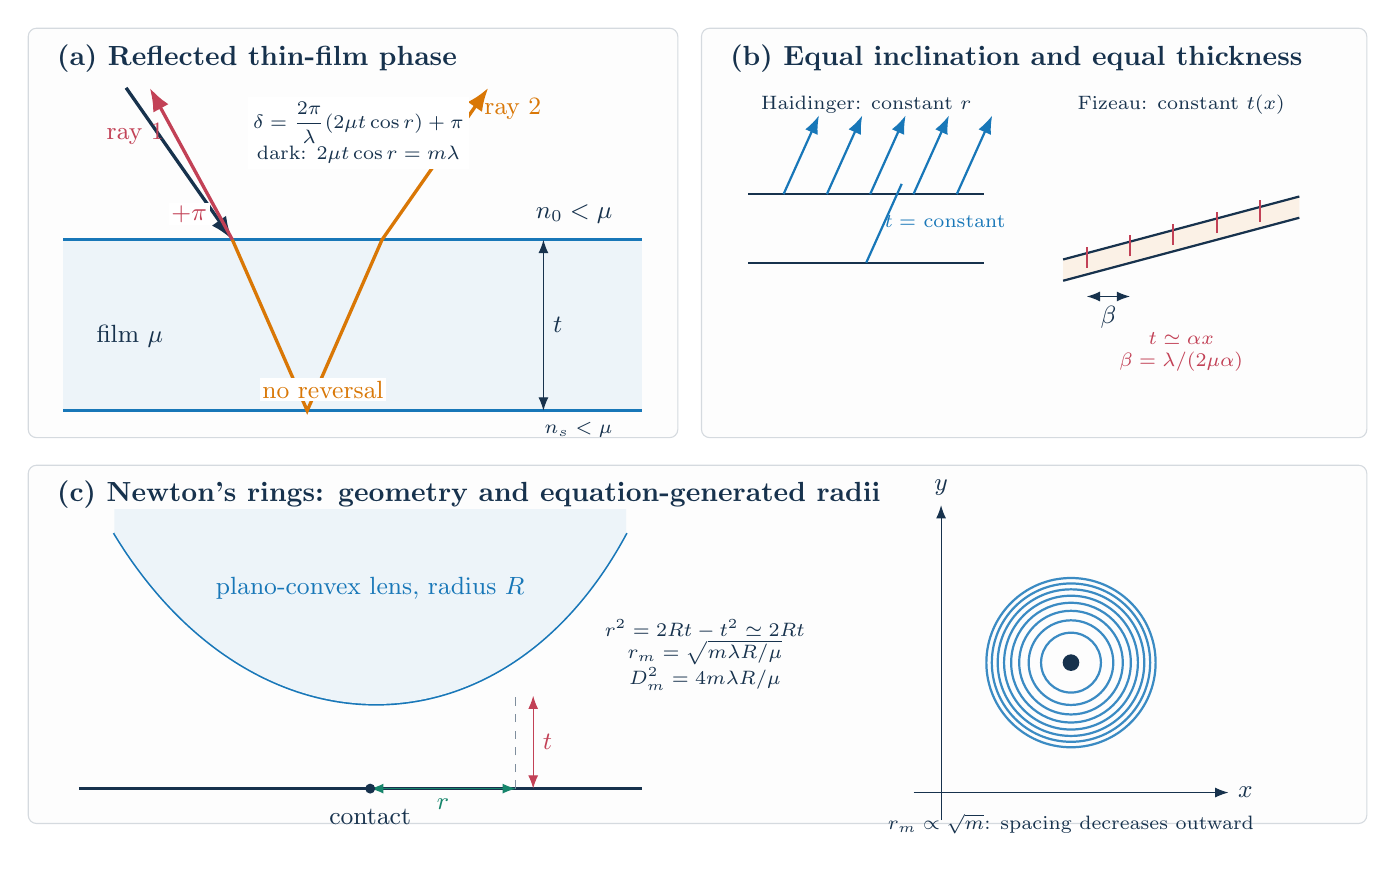
\begin{tikzpicture}[font=\small,>=Latex]
\tikzset{panel/.style={draw=ink!18,rounded corners=3pt,fill=ink!1}}

\node[panel,minimum width=8.25cm,minimum height=5.2cm,anchor=south west] at (0,4.9) {};
\node[font=\bfseries,ink,anchor=west] at (.25,9.72) {(a) Reflected thin-film phase};
\fill[blue!8] (.45,5.25) rectangle (7.8,7.42);
\draw[very thick,blue] (.45,7.42)--(7.8,7.42);
\draw[very thick,blue] (.45,5.25)--(7.8,5.25);
\node[ink,anchor=south east] at (7.55,7.50) {$n_0<\mu$};
\node[ink,anchor=west] at (.75,6.20) {film $\mu$};
\node[ink,font=\scriptsize,anchor=north east] at (7.55,5.22) {$n_s<\mu$};
\coordinate (A) at (2.6,7.42);
\coordinate (B) at (3.55,5.25);
\coordinate (C) at (4.50,7.42);
\draw[->,ink,very thick] (1.25,9.35)--(A);
\draw[->,red,very thick] (A)--(1.55,9.35) node[pos=.7,left] {ray 1};
\draw[->,orange,very thick] (A)--(B)--(C)--(5.85,9.35) node[pos=.86,right] {ray 2};
\draw[<->,ink] (6.55,5.25)--(6.55,7.42) node[midway,right] {$t$};
\node[red,fill=white,inner sep=1pt] at (2.05,7.75) {$+\pi$};
\node[orange,fill=white,inner sep=1pt] at (3.75,5.52) {no reversal};
\node[align=center,font=\scriptsize,ink,fill=white,inner sep=2pt] at (4.20,8.78)
  {$\delta=\dfrac{2\pi}{\lambda}(2\mu t\cos r)+\pi$\\
   dark: $2\mu t\cos r=m\lambda$};

\node[panel,minimum width=8.45cm,minimum height=5.2cm,anchor=south west] at (8.55,4.9) {};
\node[font=\bfseries,ink,anchor=west] at (8.80,9.72) {(b) Equal inclination and equal thickness};
\begin{scope}[shift={(9.10,5.35)}]
  \node[ink,font=\scriptsize] at (1.55,3.78) {Haidinger: constant $r$};
  \draw[thick,ink] (.05,2.65)--(3.05,2.65);
  \draw[thick,ink] (.05,1.78)--(3.05,1.78);
  \foreach \x in {.50,1.05,1.60,2.15,2.70}{
    \draw[->,blue,thick] (\x,2.65)--++(.45,1.0);
  }
  \draw[blue,thick] (1.55,1.78)--++(.45,1.0);
  \node[blue,font=\scriptsize] at (2.55,2.3) {$t=$ constant};
  \begin{scope}[shift={(4.0,0)}]
    \node[ink,font=\scriptsize] at (1.55,3.78) {Fizeau: constant $t(x)$};
    \fill[orange!10] (.05,1.55)--(3.05,2.35)--(3.05,2.62)--(.05,1.82)--cycle;
    \draw[thick,ink] (.05,1.55)--(3.05,2.35);
    \draw[thick,ink] (.05,1.82)--(3.05,2.62);
    \foreach \x in {.35,.90,1.45,2.00,2.55}{
      \draw[red,thick] (\x,1.62+.2667*\x)--++(0,.27);
    }
    \draw[<->,ink] (.35,1.35)--(.90,1.35) node[midway,below] {$\beta$};
    \node[red,font=\scriptsize,align=center] at (1.55,.65)
      {$t\simeq\alpha x$\\$\beta=\lambda/(2\mu\alpha)$};
  \end{scope}
\end{scope}

\node[panel,minimum width=17cm,minimum height=4.55cm,anchor=south west] at (0,0) {};
\node[font=\bfseries,ink,anchor=west] at (.25,4.18) {(c) Newton's rings: geometry and equation-generated radii};
\begin{scope}[shift={(.65,.45)}]
  \draw[very thick,ink] (0,0)--(7.15,0);
  \draw[very thick,blue] (0.45,3.25) .. controls (2.2,.35) and (5.4,.35) .. (6.95,3.25);
  \fill[blue!8] (0.45,3.25) .. controls (2.2,.35) and (5.4,.35) .. (6.95,3.25)
      --(6.95,3.55)--(.45,3.55)--cycle;
  \coordinate (O) at (3.70,0);
  \coordinate (P) at (5.55,0);
  \draw[dashed,ink!55] (P)--(5.55,1.18);
  \draw[<->,red] (5.77,0)--(5.77,1.18) node[midway,right] {$t$};
  \draw[<->,green] (O)--(P) node[midway,below] {$r$};
  \fill[ink] (O) circle (1.8pt) node[below=4pt] {contact};
  \node[blue] at (3.7,2.55) {plano-convex lens, radius $R$};
  \node[align=center,font=\scriptsize,ink] at (7.95,1.7)
    {$r^2=2Rt-t^2\simeq2Rt$\\
     $r_m=\sqrt{m\lambda R/\mu}$\\
     $D_m^2=4m\lambda R/\mu$};
\end{scope}
\begin{scope}[shift={(13.25,2.05)}]
  \fill[ink] (0,0) circle (3pt);
  \foreach \m in {1,...,8}{
    \draw[blue!85,thick] (0,0) circle ({.38*sqrt(\m)});
  }
  \draw[->,ink] (-2.0,-1.65)--(2.0,-1.65) node[right] {$x$};
  \draw[->,ink] (-1.65,-2.0)--(-1.65,2.0) node[above] {$y$};
  \node[font=\scriptsize,ink] at (0,-2.05) {$r_m\propto\sqrt m$: spacing decreases outward};
\end{scope}
\end{tikzpicture}
\end{document}
